\begin{Exercise}[title=Déviation d'un électron par un champ électrique]
  \begin{minipage}{.45\linewidth}
    Le but de cet exercice est de déterminer la déviation d'une particule chargée par un champ électrique uniforme, tel qu'elle apparaît dans l'expérience de Thomson.

    On s'intéresse à un électron arrivant dans une zone où il existe un champ éléctrique $\vec{E}$ avec une vitesse $\vec{v_0}$ perpendiculaire à $\vec{E}$. On note que le champ déflecteur n'est présent que dans une zone limitée de l'espace de largeur $a$.
    \begin{enumerate}
    \item Calculer les vecteurs positions et vitesse à la sortie de la zone où s'applique le champ $\vec{E}$
    \item En déduire l'angle de déflexion $\theta$ dû à l'action du champ électrique sur l'électron.
    \item calculer la déflexion $d$
    \end{enumerate}
  \end{minipage}\hspace{.05\linewidth}
  \begin{minipage}{.45\linewidth}
    \includegraphics[width=\linewidth]{thomson.png}
  \end{minipage}
\end{Exercise}
\begin{Answer}
		\Question
		\[\begin{cases}
		\ddot{x} =\frac{-eE}{m}\\
		\ddot{y} =0\\
		\end{cases} \implies
		\begin{cases}
		\dot{x} = \frac{-eE}{m}t\\
		\dot{y} = v_0
		\end{cases} \implies\\
		\begin{cases}
		x = \frac{-eE}{2m}t^2 + \\
		y = v_0  t
		\end{cases}
		\]
		La particule quitte la zone ou règne le champ en $y_1=a$ à l'instant $t_1 = a/v_0 $  au point d'abscisse $x_1 = \frac{-eEa^2}{2mv_0^2}$. on a en ce point $\dot{x} = \frac{-eEa}{mv_0}$
		\Question Dans la zone suivante , plus de champ, trajectoire rectiligne uniforme et on a $\tan\theta = \frac{\dot{x}}{\dot{y}} = \frac{eEa}{mv_0^2}$
		\Question Alors à une distance $L >> a$ on a:
		$d = \frac{eEa}{mv_0^2}(a/2+L) \simeq \frac{eEaL}{mv_0^2}$
\end{Answer}
